\documentclass{beamer}
\usepackage{scrextend}
\usepackage{amsfonts}
%\usepackage[T1]{fontenc}
\usepackage{booktabs}
\usepackage[latin1]{inputenc}
\usepackage{graphicx}
\usepackage{mathtools}
\usepackage{multimedia}
\usepackage{url}
\usepackage{tikz}
\usepackage{pstricks,pst-node}
%Packages Tableaux
\usepackage{tabularx} %Tableaux
\usepackage{multirow} %Gestion des lignes
\usepackage{multicol} %Gestion des colones
\usepackage{fancybox} %Boites
\usepackage{multicol} %Colonnes
\usepackage{array} %Tableaux maths
\usepackage{fancybox}
\usetikzlibrary{arrows} 
\usetheme{Ilmenau}



\title[Monthly Meeting: June]{Inverse Procedural Generation of Geological Stories}
\author{Garcia Maxime}
%\institute{Mosig GVR}
%\date{January 2016}


\begin{document}

	
    \begin{frame}[label=(intro)]
	\titlepage
    \end{frame}
	
	
	\begin{frame}
	\frametitle{Today's agenda}
	\begin{itemize}
	\setbeamertemplate{itemize item}[ball]
	\item Unit tests - Presentation of event undos
	\setbeamertemplate{itemize item}[ball]
	\item Story Telling Management
	\setbeamertemplate{itemize item}[ball]
	\item Chartreuse Solving Sequence

	\end{itemize}
	\end{frame}
	
	
	\section{Unit Tests}
	
	\begin{frame}
	\frametitle{Events To Undo}
    \begin{itemize}
    \item Sedimentation $\rightarrow$  UnSediment (2 ways of solving UnSediment Event)
    \item Erosion $\rightarrow$  UnErode (6 ways of solving UnErode Event)
    \item Fold $\rightarrow$  UnFold (3 ways of solving UnFold Event)
    \item Fault $\rightarrow$  UnFault (1 way of solving UnFault Event)
    \end{itemize}
    \end{frame}
    
    \begin{frame}
	\frametitle{Simulation coefficients}
    \begin{itemize}
    \item Time step $dt = 0.01$
	\item Torsion $(Tk) = 20$
	\item Stiffness $(k) = 10000$ for every materials 
	\item Friction $(f) = 0.2$ for every materials 
	\item Fold forces amplitude $= 0.001*k$
    \end{itemize}
    \end{frame}
    
	\begin{frame}
	\frametitle{UnSediment Event}
	\begin{itemize}
	\item We can either UnSediment one unit or every unit of the same material
	\item The user can specify how long the event should last 
	\item Principle: we progressively decrease the equilibrium length of vertical springs 
	\item Units will loose gradually width
	\item Units are erased at the end of the desired time
	\item Possibly use inverse torsion dynamic to prevent unit self intersections
	\end{itemize}
	\url{UnSediment.flv}
	\end{frame}
	
	\begin{frame}
	\frametitle{UnErode Events}
	\begin{itemize}
	\item 6 ways of un-doing the erosion event for six cases
	\item Fill gaps between two units of the same material in the same block
	\item Fill unit parts which are in a gap between two more recent unit of the same material
	\item Fill youngest units which are at the surface
	\item Fill units sides
	\item Fill gap between two units of the same material in neighbouring blocks (one unit on the left block and the other on the right)
	\item Fill units which have interlayer at the surface just below them
	\end{itemize}
	\end{frame}
	
	\begin{frame}
	\frametitle{UnErode Event: gap between two units}
	\begin{itemize}
	\item Principle: merge the two units by creating a boundary if necessary using Hermite curves
	\item Preserve the continuity of the units bending
	\end{itemize}
	\url{unErodeMerge.flv}
	\end{frame}		
	
	\begin{frame}
	\frametitle{UnErode Event: unit part in a gap between two units}
	\begin{itemize}
	\item Principle: fill the gap using Hermite curve joining the extremities of the gap
	\item Preserve the continuity of the unit bending 
	\item Allow to fill lacking matter even if there are no concavities which make the erosion obvious.
	\end{itemize}
	\url{unErodeSurface.flv}
	\end{frame}	
	
	\begin{frame}
	\frametitle{UnErode Event:  youngest units which are at the surface}
	\begin{itemize}
	\item Principle: fill the concavities of the surface using also Hermite curves
	\item Preserve the continuity of the unit bending 
	\item Concavities are detected using a parametrisation of the surface curve.
	\end{itemize}
	\url{unErodeYoungest.flv}
	\end{frame}	
	
	\begin{frame}
	\frametitle{UnErode Event: unit sides}
	\begin{itemize}
	\item Principle: fill the concavities of the units' sides but not all of them
	\item Starting by the upper corners of the unit we try to add matter going progessively at unit the bottom 
	\item We stop the filling when the curve becomes fully convex (see video).
	\item This is detected when drawing a string from the corner to the side particles always intersect the unit( see video).
	\end{itemize}
	\url{unErodeSide.flv}
	\end{frame}
	
	
	\begin{frame}
	\frametitle{UnErode Event: gap between two units of neighbouring blocks}
	\begin{itemize}
	\item Principle: merge the two units by creating a boundary if necessary using Hermite curves
	\item Preserve the continuity of the units bending
	\item Same thing than in the same block case but the two blocks have now a unit in common and the blocks' mass-spring system is not regenerated
	\end{itemize}
	\url{unFaultUnErode.flv}
	\end{frame}	

	\begin{frame}
	\frametitle{UnErode Event: units with surface interlayers below them}
	\begin{itemize}
	\item Principle: add matter to the unit where there are surface interlayer of the unit just below them
	\item The unit below is older and matter will be added conserving the current width of the unEroded unit
	\item the width might be increased if the below unit is stringly folded.
	\end{itemize}
	\url{unFaultUnErode.flv}
	\end{frame}		
	
	\begin{frame}
	\frametitle{UnFold Event}
	\begin{itemize}
	\item Principle: add external forces either to a block,a unit or a particle
	\item Allow to apply uniform and non uniform forces on a block
	\item Duration time can be set by the user
	\end{itemize}
	\end{frame}		
	

	\begin{frame}
	\frametitle{UnFault Event}
	\begin{itemize}
	\item Decomposed into three sequences of events
	\item First possibly apply unErode event to units which are not in contact in th fault
	\item Then make the upper block sliding on the other and control the moment unit of the same material are face to face
	(unit events)
	\item Apply UnFold event on one of the block in order to close the fault
	\end{itemize}
	\url{UnFault.flv}
	\end{frame}		
	
	
	\section{Story Telling}
	
	\begin{frame}
	\frametitle{Handling the Story Telling}
	\begin{itemize}
	\item Use Event Graph to establish a time dependency between Events
	\item Use Story Graph to build the different scenarios and choose the event to play
	\item The Event Graph is generated when the drawing is loaded but can be updated during the simulation
	\item Dynamic events have been added. There are events generated when creating a new node in the story graph during the simulation . For instance they could be unErode concavities event or even unFolding events added by the user
	\end{itemize}
	\end{frame}	
		
	\begin{frame} 
    \frametitle{Event Graph example}
    \includegraphics[scale=0.4]{eventGraph.pdf}
    \linebreak
    \linebreak
    \includegraphics[scale=0.4]{timeArrowRight.pdf}
    \end{frame}
    
    \begin{frame} 
    \frametitle{Story Graph example}
    \includegraphics[scale=0.4]{StoryGraph.pdf}
    \linebreak
    \linebreak
    \includegraphics[scale=0.4]{timeArrowLeft.pdf}
    \end{frame}
	
	\begin{frame}
	\frametitle{Proposing events to the user}
	\begin{itemize}
	\item Events have conditions to fulfill in order to be among the possible choices $\rightarrow$ precondition.
	\item Even if they fulfill the precondition they have a probability of occurence. If it is below a threshold the event will not be proposed $\rightarrow$  branch and bound using evaluation functions
	\item Events have conditions to fulfill in order to end $\rightarrow$  postconditions
	\end{itemize}
	\end{frame}
	
	\begin{frame}
	\frametitle{Evaluation functions examples}
	\begin{itemize}
	\item unFault $\rightarrow$  compare the side length of the two faulting blocks. The bigger the difference in side length the less the event has a chance to be proposed.
	\item unErode Unit Side $\rightarrow$  it is possible to predict the matter quantity that will be added. If it is too low the event will not be proposed
	\item unSediment and unFold events are always proposed as the sedimentation it is fully determined using only the event graph and the unFold event is added by the user as he wishes.
	\end{itemize}
	\end{frame}	
	
	\section{Chartreuse Solving Sequence}


	\begin{frame}
	\frametitle{Chartreuse Section}
	\center{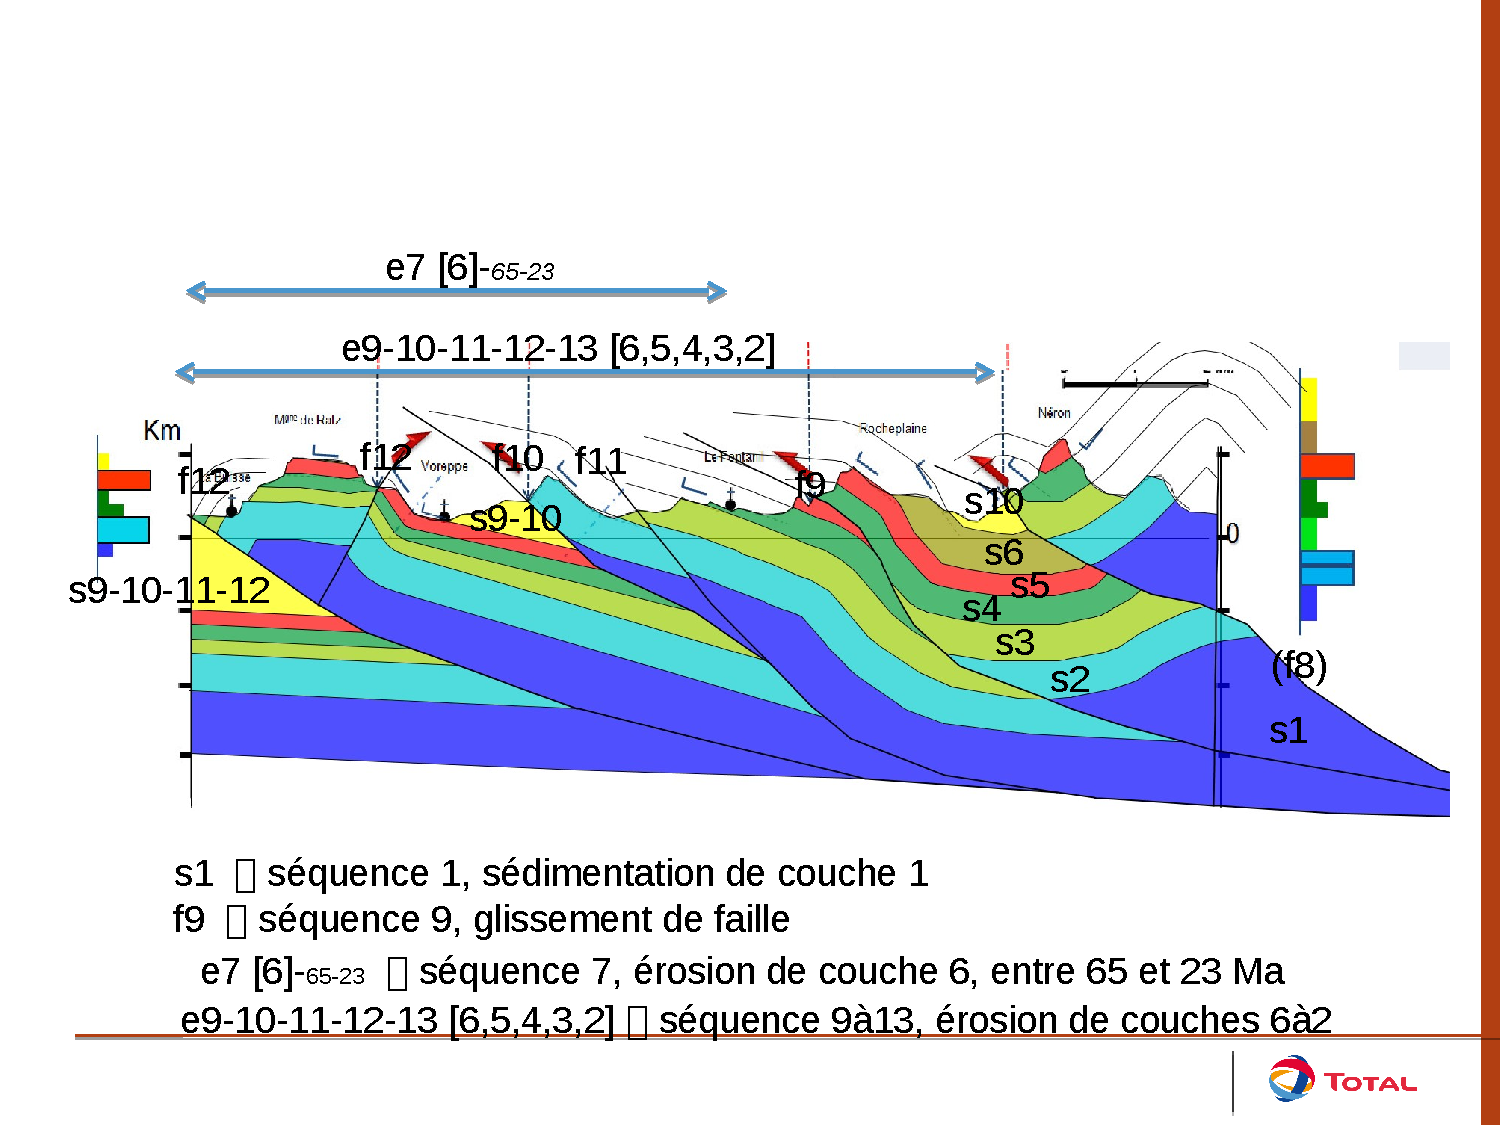
\includegraphics[scale=0.36]{Coupe_Chartreuse_rediscutee.pdf}}
	\end{frame}
	
	\begin{frame}
	\frametitle{Sequential History of Chartreuse}
	S1 sediment layer 1  $\rightarrow$ 	S2 sediment layer 2 $\rightarrow$ \\
	S3 sediment layer 3 $\rightarrow$  	S4 sediment layer 4 $\rightarrow$ \\
	S5 sediment layer 5  $\rightarrow$ 	S6 sediment layer 6 $\rightarrow$ \\
	E7 erode layer 6 $\rightarrow$  	F9 slide along fault 9 $\rightarrow$ \\
	E9 erode layer 6 continued  $\rightarrow$ 	S9 sediment layer 7 $\rightarrow$ \\
	E10 erode layer 5  	 $\rightarrow$   S10 sediment layer 7 $\rightarrow$ \\
	F10 slide along fault 10   $\rightarrow$   E11 erode layer 4 $\rightarrow$ \\
	S11 sediment layer 7   $\rightarrow$   F11 slide along fault 11 $\rightarrow$ \\
	E12 erode layer 3  $\rightarrow$    S12 sediment layer 7 $\rightarrow$ \\
	F12 slide along fault 12   $\rightarrow$   E13 erode layer 2\\
	\end{frame}	

	
\end{document}